
\chapter{Menu Tags}\label{tags_chapter}
\minitoc 


All vertices of different biological structures can be given a specific integer values (0, 1, 2, 3 ...), in order to identify them. Such integer arrays are referred to as "tag arrays". 
As stated earlier, a given unselected surface can be colored using the currently active tag array (identified by its "name"), if that surface contains a tag array of that name (see also Fig. \ref{4color_modes}-B p.\pageref{4color_modes}). To do so, the array display mode button must be pressed (
\includegraphics[scale=0.7]{images/04/show_color_scale.png}), and a \textbf{tag} array must be selected as the currently active array (ex:
\includegraphics[scale=0.5]{images/04/scalarcombo_tag.png}). The way tag arrays are translated into colors can be set up using tag maps, also referred to as "Lookup tables" (LUT) or color transfer functions. \\
Contrary to "scalar arrays" (see preceding section), tags are usually drawn manually with "painting tools". \\
For convenience purposes, as selected surfaces are drawn "grey" in MorphoDig, unselected surfaces objects can be tagged (tagging uniform "grey" objects without visual feedback would be uneasy). Tagging is the only way to modify an unselected surface in MorphoDig. \\
In order to be able to edit tags on a surface, the most common way is to create a new empty tag array for this surface (see section \ref{empty_tag_array} p. \ref{empty_tag_array} for further details). You may read section \ref{tag_starting_guide} p.\pageref{tag_starting_guide} for a quick tagging starting guide. 


\section{Open Tags window}
The "Tags" window can be also opened by clicking on "
\includegraphics[scale=0.7]{images/04/tag_edit.png}" (see Fig. \ref{tags_window}). The Tags window contains most options related to tags. The active tag array can be chosen here, as well as the active tag map. Tag maps (name, color, opacity of different biological structures) can be defined and modified here as well. The currently used tag tool is also chosen in this window (pencil "
\includegraphics[scale=0.7]{images/12/pencil.png}", paint bucket "
\includegraphics[scale=0.7]{images/12/paint_bucket.png}" or lasso "
\includegraphics[scale=0.7]{images/12/lasso.png}"). 


\begin{figure}
  \centering
  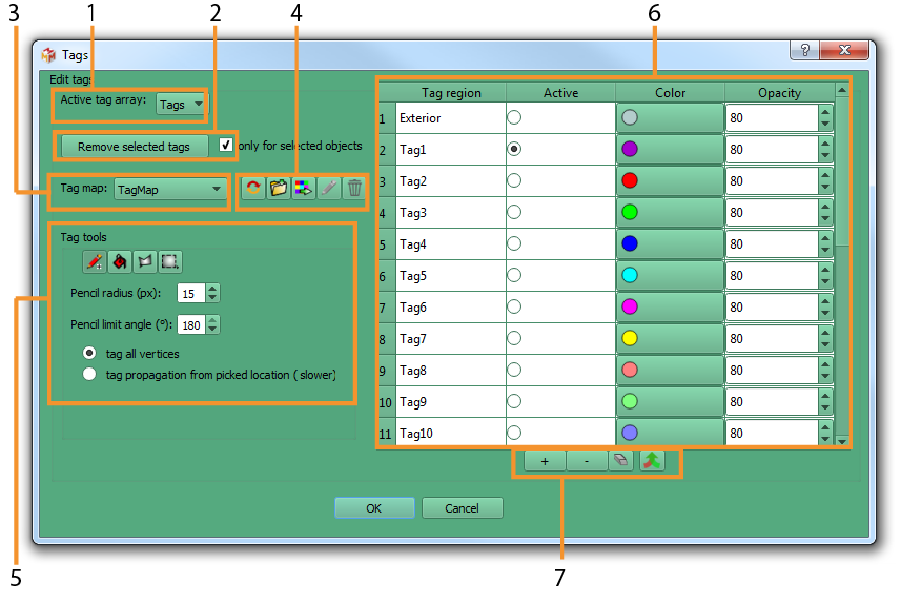
\includegraphics[scale=1]{images/12/tags_window2.png}
\caption{Tags window. This window is divided in different subsections. \textbf{1)} choose current active tag array.  \textbf{2)} the active tag array can be deleted from selected/all surface objects in this sections. \textbf{3)} choose current active tag map, which transforms integer values into color and opacity on the screen. \textbf{4)} operations on the active tag map (from left to right). a: reinitialize tag map. b: Add tag map to presets = duplicate current active tag map and create a new custom tag map. c: export tag map(s) inside a .TAG or .TGP file. d: change active color map name (only possible for custom tag maps). d: delete active color map (only possible for custom tag maps). \textbf{5)} active tag tools (from left to right): a: pencil. b: paint bucket. c: lasso tag. d: pencil radius size (in pixels rendered on the screen).  \textbf{6)} The tag map table: each line of this table is associated with an integer (exterior: 0; Tag1: 1 etc.), a color and an opacity. The active tag tools will paint a surface using the active tag. \textbf{7)} modification controls of the active tag map (from left to right). a: add a line to tag map table. b: remove last line from tag map table. c: reset active tag (merge with Tag 0 = Exterior). d: merge two tags.}	
\label{tags_window}
 \end{figure}


\noindent



\section{Create new empty tag array for each selected surface}\label{empty_tag_array}

\begin{minipage}{0.5\textwidth}
This option will create a new "empty" tag array (the name of this new array is given by the user). "Empty", in this context, means that all vertices are assigned to the "Exterior" tag (tag=0).\end{minipage} 
\begin{minipage}{0.5\textwidth}\centering
  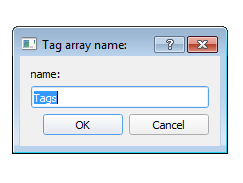
\includegraphics[scale=0.5]{images/12/empty_tag_array.png}
 \captionof{figure}{Creating a new tag array}
 \end{minipage} 



\section{Create new tag array based on currently displayed colors for each selected surface}
Advice: \textbf{do not} use this method on surfaces displayed with \textbf{color gradients}. This option usually only makes sense when distinct colors are displayed (typically: less than 30).\\
This option (see Fig. \ref{rgb_conversion}) may be useful when you just have opened a .ply file already containing RGB colors (for instance, let us suppose that you have painted a surface using MeshLab software, and that you wish to convert those colors into tags). RGB colors contained in .ply files are inserted inside the RGB array when opened with MorphoDig. This option is not restricted to RGB arrays contained inside .ply files though: it is also possible to convert any displayed color (such as scalar color rendering via a discretized color table) into a tag value. 

\begin{figure}
  \centering
  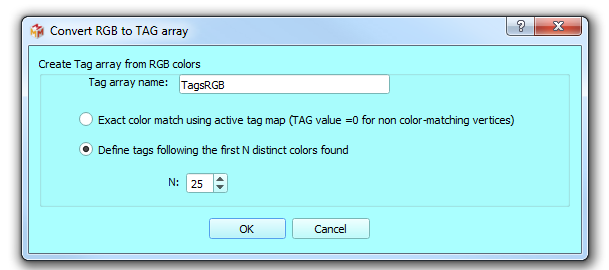
\includegraphics[scale=0.5]{images/12/tags_from_rgb.png} 
	\caption{Create Tag array from RGB array.}
\label{rgb_conversion}
\end{figure}
Two main ways to convert currently displayed colors are available :\\
\textbf{\underline{1) Exact color match using active tag map}}\\
$\rightarrow$ In that case, in order to be given a tag value other than Tag 00, a vertex must satisfy the following condition: its RGB scalar value should match one of the colors defined in the "Tags options" window for the active tag map. If a vertex does not satisfy this condition, it is given the Tag 00 value (=exterior).\\
\textbf{\underline{2) Define tags following the first N distinct colors found}}\\
$\rightarrow$ In that case the following sequence of operations is performed:\\
a) Important: MorphoDig re-initializes the currently active tag map. If you have spent time to define colors and labels on the currently active tag map, it is strongly advised to save the active tag map inside a .TAG or .TGP file in order to be able to re-load it later. Otherwise, your work will be lost.\\
b) MorphoDig inspects the RGB display color of all the vertices of opened surfaces. When meeting a new color, if the active tag map contains less than "N" lines, MorphoDig inserts a new line inside the active tag map (of that color), and associates the current vertex id to this new tag id entry. All vertices of that same color will be associated to that id. If the color of the vertex is "new" and the maximum number of allowed entries in the tag map (N) has been reached, the vertex is associated with "tag id=0".\\
Method \#1 will work perfectly if you are used to work with a well-defined set of colors on 3D surfaces, and have spent time to define a tag map with those colors.\\
Method \#2 is much faster, but may lead to messy results: tag entries in the tag map will be ordered in a non-biological way.\\

Also remember not to use these methods when surfaces are displayed with color gradients. An example of use of method 2 is shown in Fig. \ref{rgb_conversion_example} p.\pageref{rgb_conversion_example}.


\begin{figure}
  \centering
  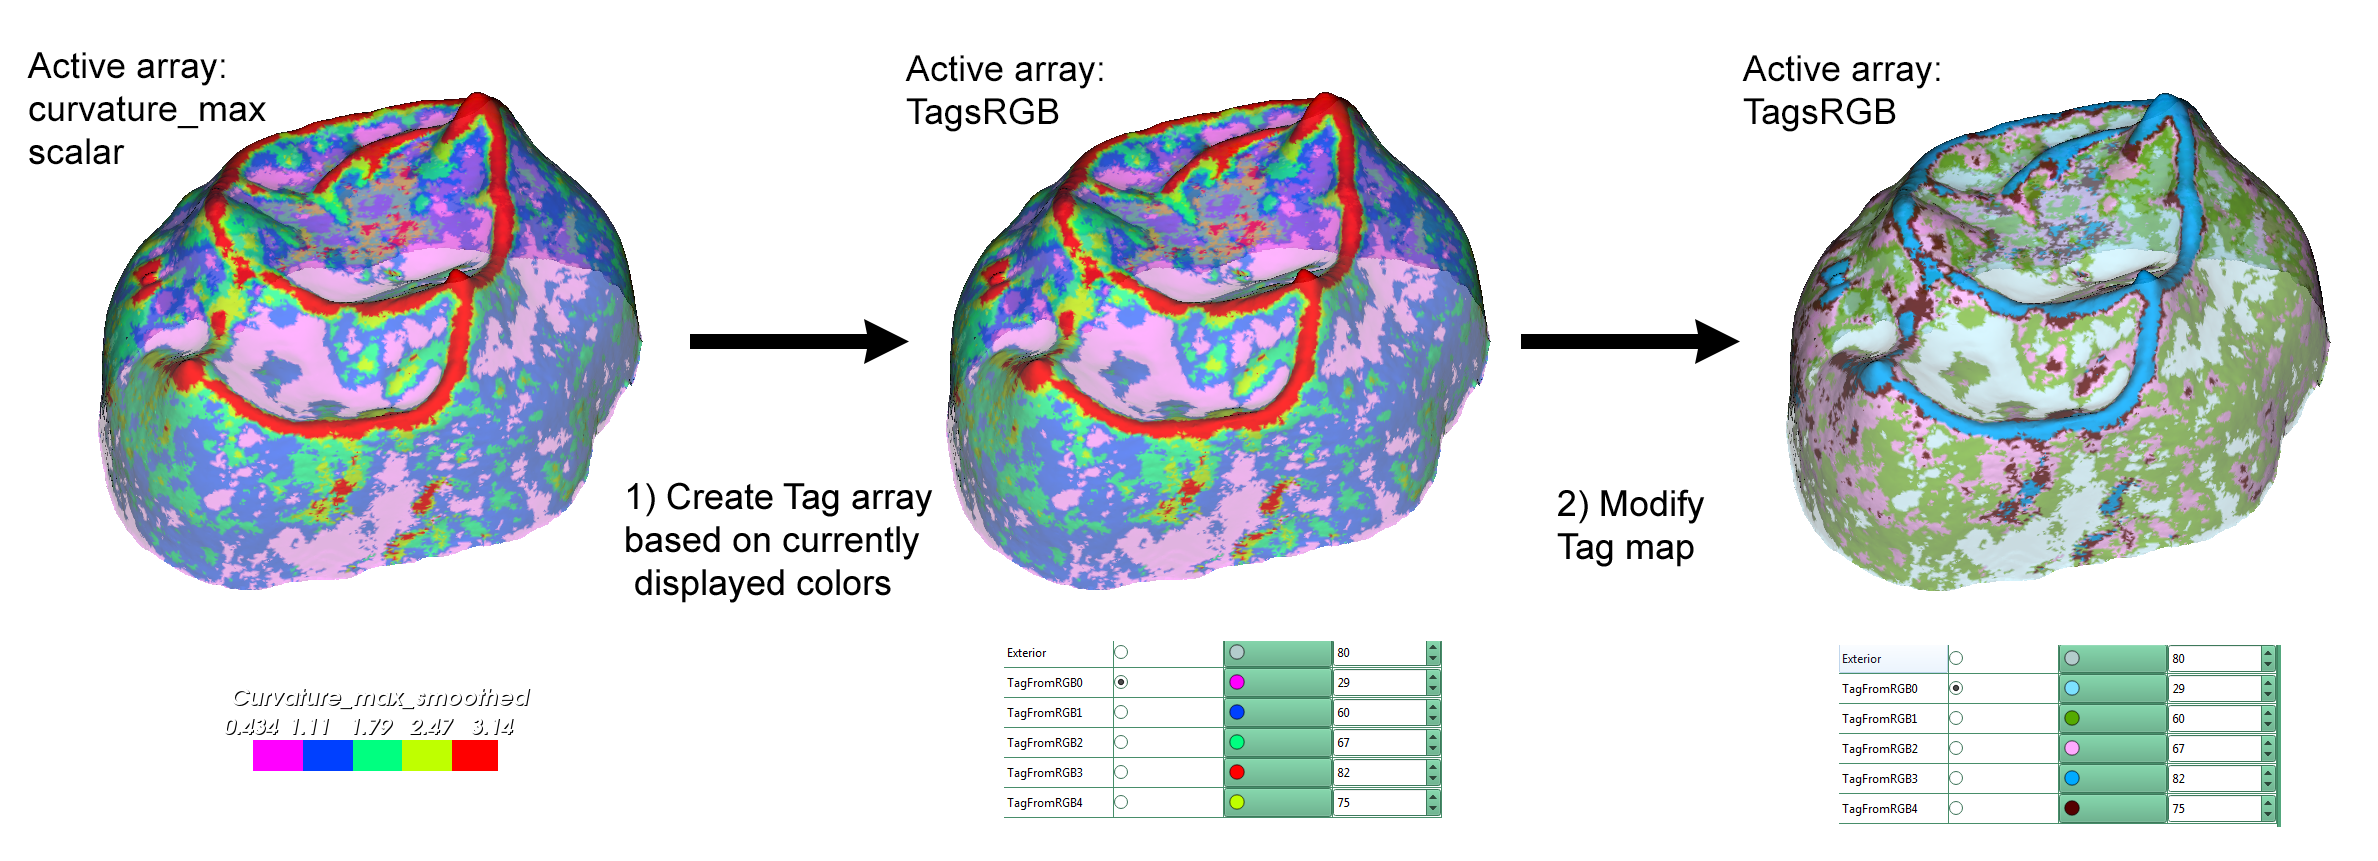
\includegraphics[scale=0.2]{images/12/tags_from_rgb_example.png} 
	\caption{Example of automatic tag array creation based on displayed color of scalars. Note here that the scalar array (minimal curvature) is displayed using a \textbf{discretized color table} set up with a reasonably small number of colors (5 here). Specimen: enamel dentine junction (EDJ) of the second superior molar of a medieval human from Sains-en-Gohelle (France). Image credit: Mona Le Luyer.}
\label{rgb_conversion_example}
\end{figure}


\section{Create new tag array based on connectivity for each selected surface}

This option involves vtkPolyDataConnectivityFilter. This option will retrieve all non-connected regions of selected surfaces and assign to each of them a unique Tag id (see for instance Fig. \ref{tag_connected} p.\pageref{tag_connected}).
\begin{figure}
  \centering
  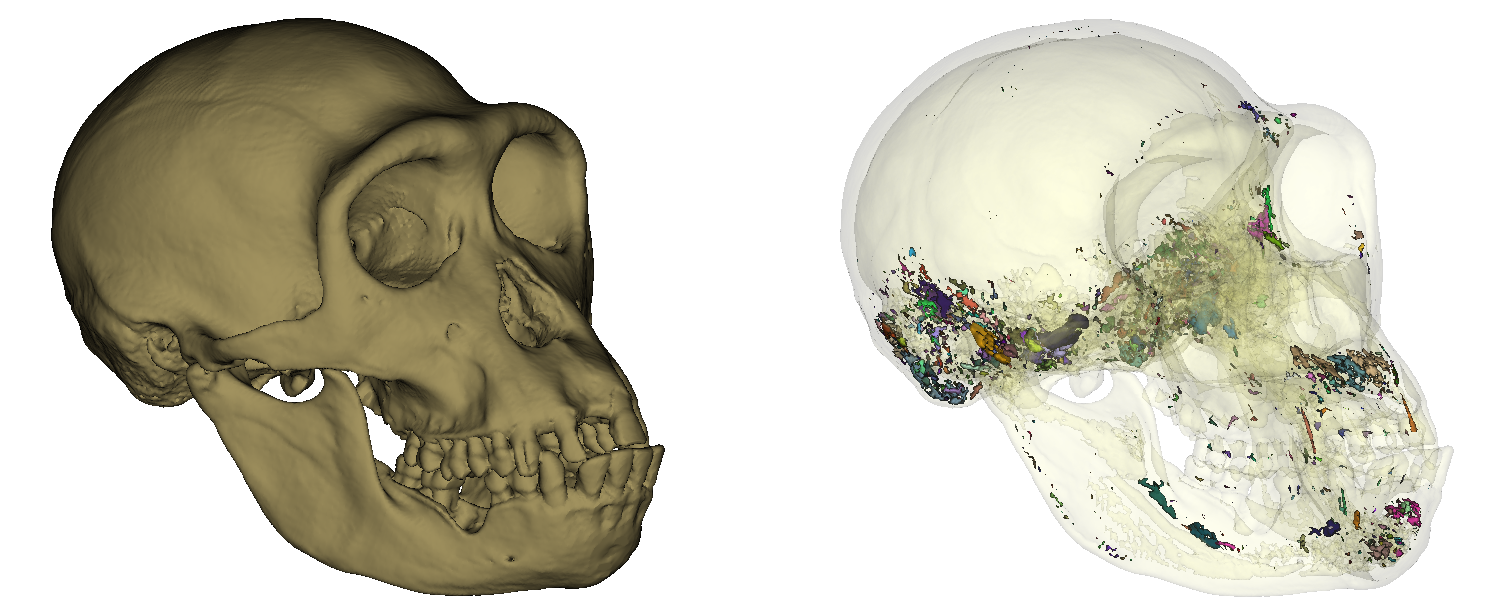
\includegraphics[scale=0.28]{images/12/connectivity_tags.png} 
	\caption{Example of tag array based on surface connectivity. Left: original surface representing the skull of the holotype specimen of \textit{Pan paniscus}. Right: a tag array ware created based on the output of the connectivity procedure: a large large number (>1000) of non connected regions was found and each was tagged. The largest region (cranium and mandible) is displayed with an opacity of 10\%, and the >1000 others with an opacity of 100\%. }
\label{tag_connected}
 
\end{figure}


\section{Tagging with MorphoDig: a quick starting guide}\label{tag_starting_guide}
\textbf{\underline{}}\\
\textbf{1: Make sure that your surface contains a Tag array}: for instance, you may create a new empty tag array for this surface (see section \ref{empty_tag_array} p. \ref{empty_tag_array} for further details). Select this tag array as the currently active array.\\\\
\noindent
\textbf{2: Open the Tags window}: a: if not already active, select desired active Tag. b: choose a tag tool (pencil "
\includegraphics[scale=0.7]{images/12/pencil.png}", paint bucket "
\includegraphics[scale=0.7]{images/12/paint_bucket.png}" or lasso "
\includegraphics[scale=0.7]{images/12/lasso.png}").  \\\\
\noindent
\textbf{3: Tag in MorphoDig's main window.} \\ a:when using the pencil "
\includegraphics[scale=0.7]{images/12/pencil.png}" or the paint bucket "
\includegraphics[scale=0.7]{images/12/paint_bucket.png}", you have two options:\\
 "T" pressed +left click: allows color override\\
 "T" pressed +right click: does not allow color override (see below for explanations of what color override is)\\
b: when using the lasso, maintain mouse left click pressed and draw a contour of the region which should be tagged.



\subsection{Pencil tag tool}

\includegraphics[scale=0.7]{images/12/pencil.png}\\
\textbf{Pencil tag tool controls:}\\
"T" pressed + left mouse click : tags the selected surface using currently active tag.\\
"T" pressed + right click : tags the selected surface using currently active tag \textbf{without color override}. Tag propagation will start at the picked vertex of a given color, but will stop when meeting another color different from that of Tag 0 (usually assigned to "exterior").\\

\textbf{Pencil tag special option:}\\
\noindent
pencil tag size (in number of pixels) on the screen can be modified in the Tags window.



\subsection{Paint bucket tag tool}

\includegraphics[scale=0.7]{images/12/paint_bucket.png}\\
\textbf{Paint bucket tag tool controls:}\\
"T" pressed + left mouse click : tags the selected surface using currently active tag.\\
"T" pressed + right click : tags the selected surface using currently active tag \textbf{without color override}. Tag propagation will start at the picked vertex of a given color, but will stop when meeting another color different from that of Tag 0 (usually assigned to "exterior").\\
 
When surfaces contain a lot of disconnected regions in space (for instance: the skeleton of a fetus), the paint bucket tool can be usefull to paint each disconnected element one by one in one mouse click. But be careful if your all regions of your surface are connected together: when using "T" + left click ("color override" allowed), as it will paint the whole object uniformly.

\subsection{Lasso tag tool} \label{lasso_tag_section}

\includegraphics[scale=0.7]{images/12/lasso.png}\\
Once the "lasso tag tool" button is pressed, draw the region to be tagged by dragging the mouse on the screen while maintaining the left button pressed. Then release the left mouse button. 

\subsection{Merge tags.}
\noindent
\begin{minipage}{0.5\textwidth}
Two tagged regions can be merged into a single one. All source tags will be put into target tags. See for instance Fig. \ref{merge_tags} p.\pageref{merge_tags}.\end{minipage}    
\begin{minipage}{0.5\textwidth}\centering
  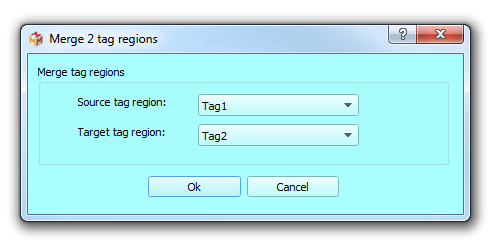
\includegraphics[scale=0.5]{images/12/merge_tags.png}
 \captionof{figure}{Merge tags window}
 \end{minipage} 
\noindent
\begin{figure}
  \centering
  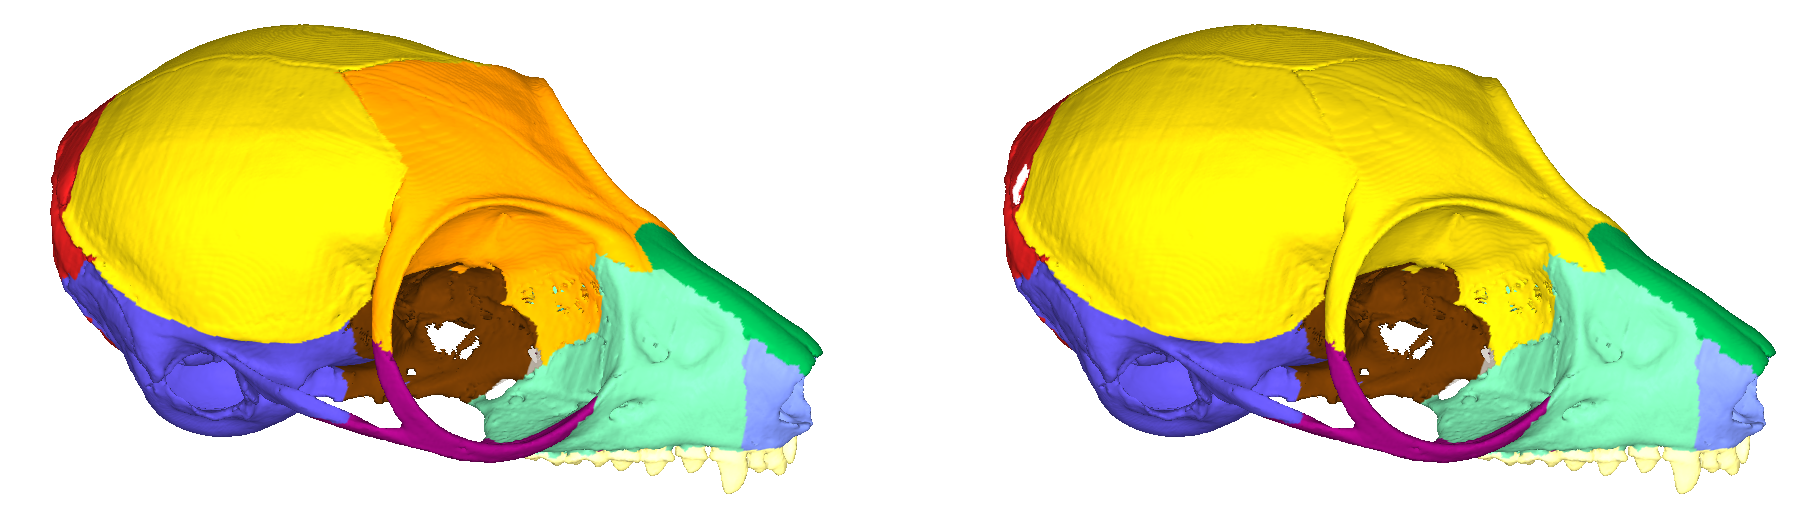
\includegraphics[scale=0.25]{images/12/merge_example.png} 
	\caption{Example of tag merging. Left : cranium of \textit{Microcebus murinus} presenting the parietal region
tagged in yellow, the frontal region tagged in orange. Right : frontal tag region was merged into
the parietal region.}
\label{merge_tags}
\end{figure}